\documentclass{article}

\usepackage{graphicx}
\usepackage{tikz}
\usepackage{tikzsymbols}
\usetikzlibrary{calc,patterns,shapes.geometric}
\pagestyle{empty}
\usepackage[margin=0pt]{geometry}
\geometry{papersize={14in,12in}}

\def\centerarc[#1](#2)(#3:#4:#5){\draw[#1] ($(#2)+({#5*cos(#3)},{#5*sin(#3)})$) arc (#3:#4:#5);}

\begin{document}
	\begin{figure}
		\centering
		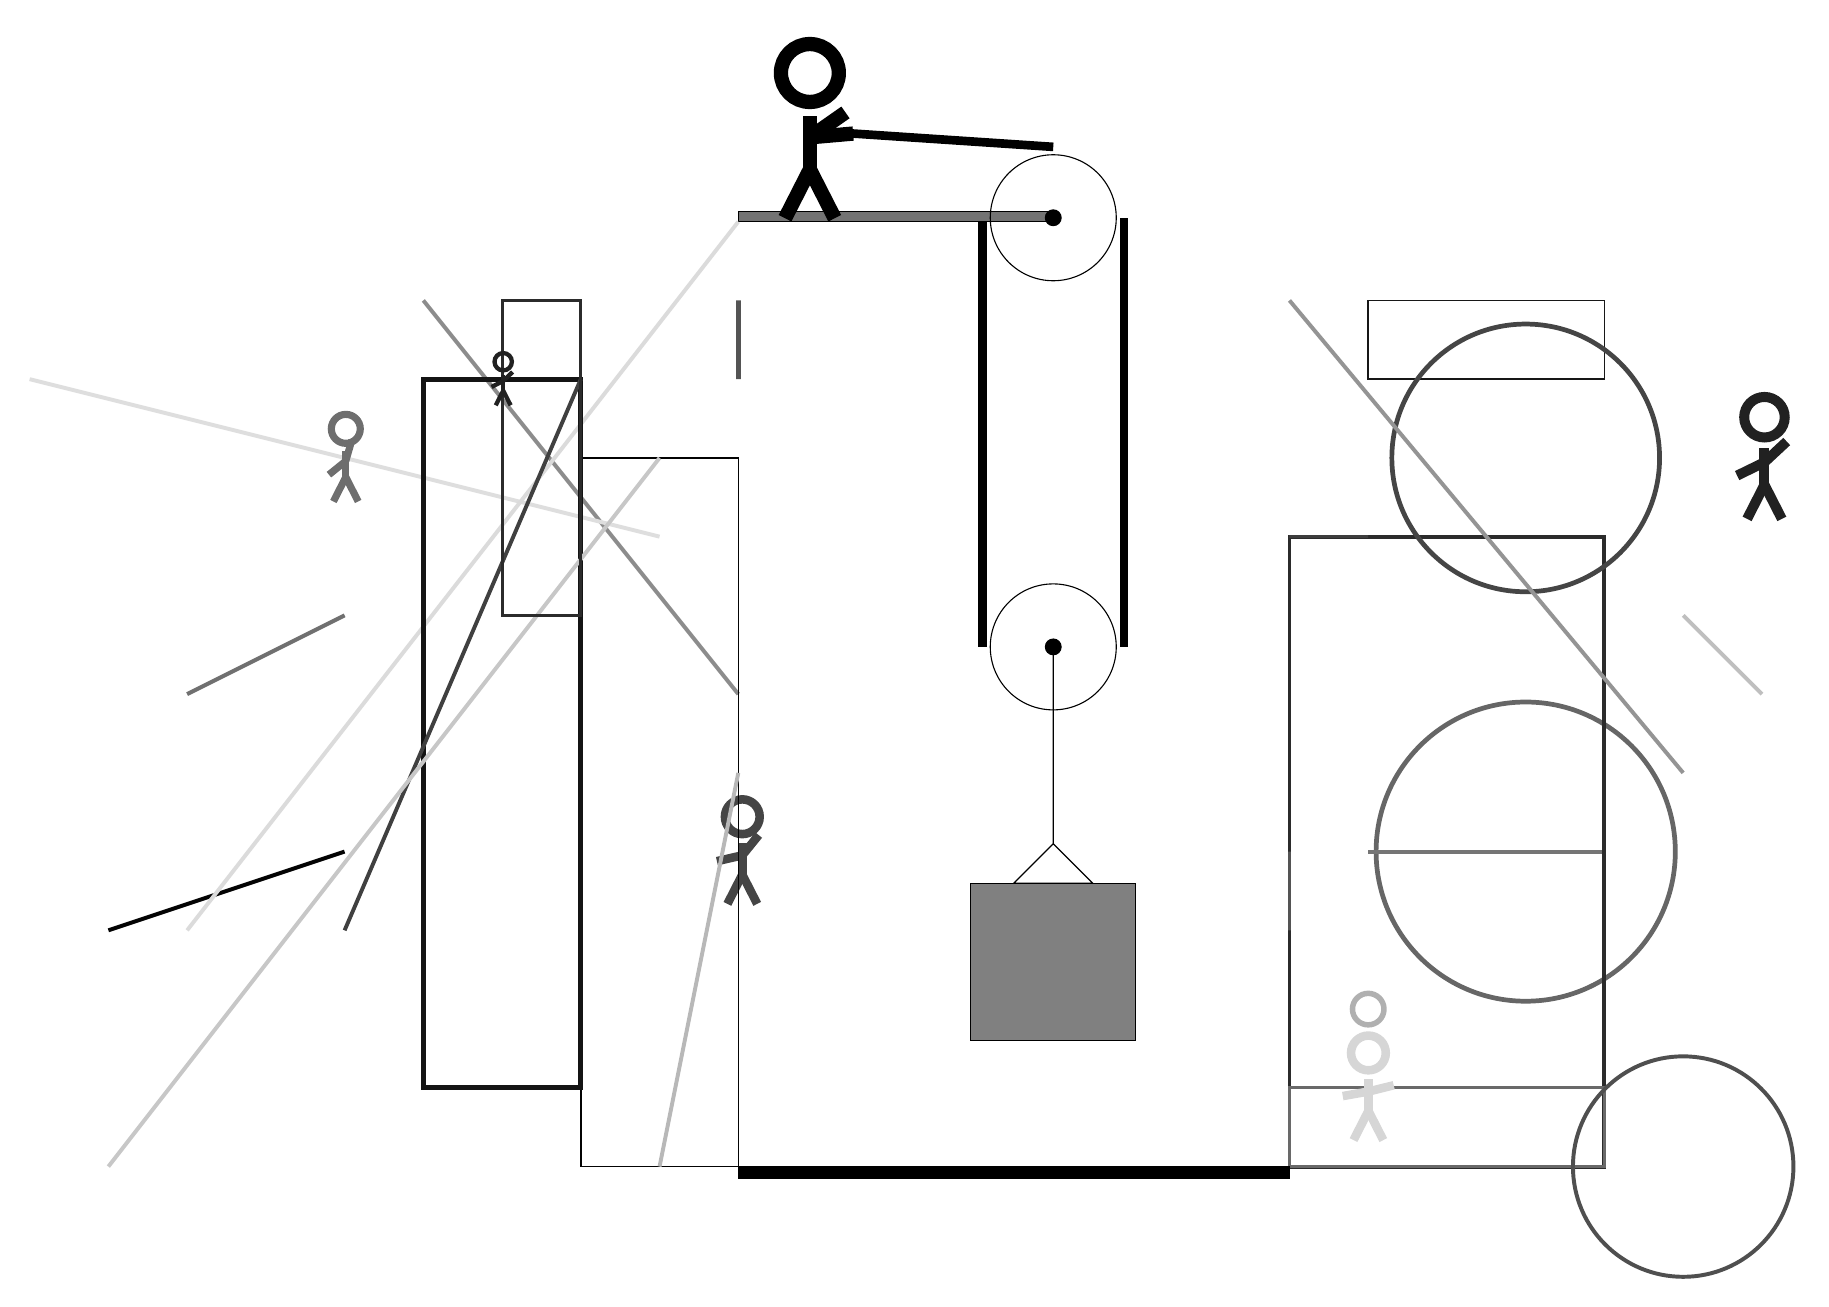
\begin{tikzpicture}
			%%%%% START %%%%%
			
			\draw[fill=black!55] (-2, 9) rectangle (2, 9.125);
			
			\draw (2, 3.6) circle (0.8);
			\draw[fill=black] (2, 3.6) circle (0.1);
			
			\draw (2, 9.05) circle (0.8);
			\draw[fill=black] (2, 9.05) circle (0.1);
			
			\draw (2, 3.6) -- (2, 1.1) -- (1.5, 0.6) -- (2.5, 0.6) -- (2, 1.1);
			\draw[fill=black!50] (0.95, 0.6) rectangle (3.05, -1.4);
			
			\draw[line width=0.7mm, color=black!67] (-2, 7) rectangle (-2, 8);
			
			\draw [line width=0.7mm, color=black!31](6, -1) circle (0.2);
			\draw [line width=0.6mm, color=black!60](8, 1) circle (1.9);
			\node[line width=0.4mm, color=black!73] at (-2, 1) {\Strichmaxerl[6][13][51]};
			\draw[line width=0.5mm, color=black!45](-2, 3) -- (-6, 8);
			\draw[line width=0.5mm, color=black!13](-3, 5) -- (-11, 7);
			\draw[line width=0.5mm, color=black!99](-7, 1) -- (-10, 0);
			\draw[line width=0.5mm, color=black!14](-2, 9) -- (-9, 0);
			\draw[line width=0.5mm, color=black!25](10, 4) -- (11, 3);
			\draw[line width=0.2mm, color=black!99] (-4, 6) rectangle (-2, -3);
			\node[line width=0.4mm, color=black!57] at (-7, 6) {\Strichmaxerl[5][39][74]};
			\draw[line width=0.5mm, color=black!54](6, 1) -- (9, 1);
			\draw[line width=0.5mm, color=black!83] (5, 5) rectangle (9, -3);
			
			\draw[line width=0.2mm, color=black!91] (6, 8) rectangle (9, 7);
			\draw[line width=0.6mm, color=black!92] (-4, -2) rectangle (-6, 7);
			\draw[line width=0.4mm, color=black!67] (5, 0) rectangle (5, 1);
			
			\draw[line width=0.4mm, color=black!59] (5, -2) rectangle (9, -3);
			\draw[line width=0.5mm, color=black!75](-7, 0) -- (-4, 7);
			\node[line width=0.2mm, color=black!16] at (6, -2) {\Strichmaxerl[6][10][14]};
			
			\draw[line width=0.5mm, color=black!28](-2, 2) -- (-3, -3);
			\draw[line width=0.5mm, color=black!56](-7, 4) -- (-9, 3);
			
			\draw[line width=0.5mm, color=black!22](-3, 6) -- (-10, -3);
			
			\draw [line width=0.6mm, color=black!73](8, 6) circle (1.7);
			\draw [line width=0.5mm, color=black!69](10, -3) circle (1.4);
			\draw[line width=0.4mm, color=black!83] (-4, 8) rectangle (-5, 4);
			
			\node[line width=0.2mm, color=black!87] at (-5, 7) {\Strichmaxerl[3][27][44]};
			
			\draw[line width=0.3mm, color=black!76] (6, 5) rectangle (5, 5);
			\draw[line width=0.5mm, color=black!42](10, 2) -- (5, 8);
			
			\node[line width=0.4mm, color=black!87] at (11, 6) {\Strichmaxerl[7][26][43]};
			
			
			\draw[line width=1.1mm] (1.1, 9) -- (1.1, 3.6);
			\centerarc[line width=1.1mm](2, 3.6)(180:360:0.9);
			\draw[line width=1.1mm](2.9, 3.6) -- (2.9, 9.05);
			\centerarc[line width=1.1mm](2, 9.05)(0:90:0.9);
			\draw[line width=1.1mm](2, 9.95) -- (-1, 10.15);
			
			\node at (-1, 10.15) {\Strichmaxerl[10][-175][35]};
			
			\draw[fill=black] (-2, -3) rectangle (5, -3.15);
			
			%%%%% END %%%%%
		\end{tikzpicture}
	\end{figure}	
\end{document}